\chapter{Data and Methodology}
\label{chap:3}
\section{Study Area}
\label{sec:3.1}
This project conducted a cross-sectional study in England, focusing on the prevalence of DM in 2022/23. We selected the Middle layer Super Output Area (MSOA) as the spatial analysis unit because it offers a moderate spatial resolution and provides more stable and smooth data distribution. Additionally, many datasets are more readily available at the MSOA level compared to the Lower layer Super Output Areas (LSOA). For example, data provided by the Office for Health Improvement and Disparities (OHID) is available at the MSOA level but not at the LSOA level (OHID, no date).

According to the statistical geography overview published by the Office for National Statistics (ONS) (no date), we understand that an MSOA typically consists of four to five LSOAs with a resident population of around 5,000 to 15,000 people. It should be noted that the MSOA boundaries were revised in 2021, increasing the number of MSOAs across England to 6,856, compared to 6,791 in 2011. As most of the datasets for this project are still based on the 2011 MSOA boundaries, this study will use the 2011 MSOA boundaries. For datasets based on the 2021 boundaries, we will use the mapping table provided by ONS (2024), with further details found in section \ref{sec:3.2.5}. Figure \ref{fig:A3.1} presents a map of England, showing the nine regions and the 2011 MSOA boundaries.

\begin{figure}[ht]
  \centering
  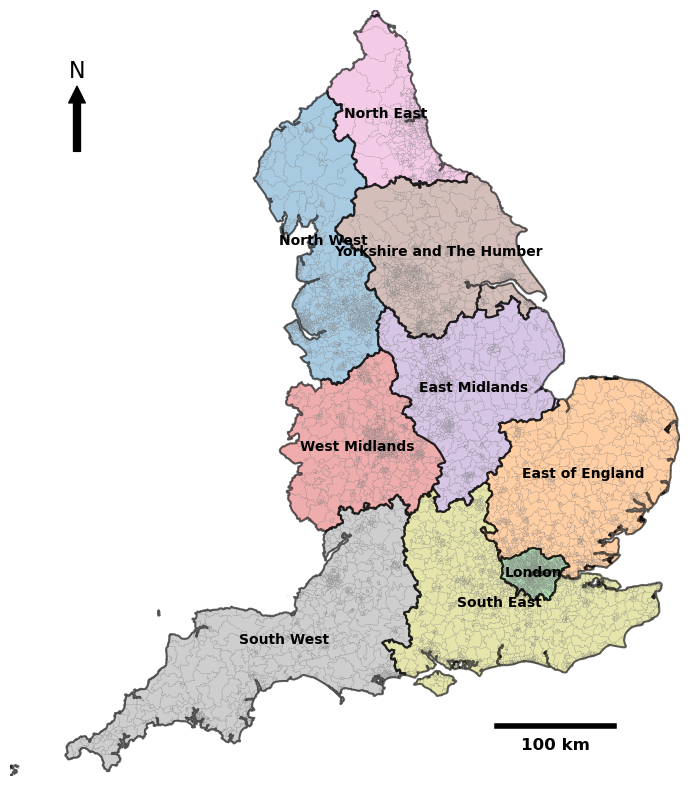
\includegraphics[width=.65\linewidth]{ucl-latex-thesis-templates-master/Image/datageo_area_1.png}
  \caption{Map of England with the boundary of nine regions and MSOAs.}
  \label{fig:A3.1}
\end{figure}%


\section{Data Sources and Data Processing}
\label{sec:3.2}
\subsection{DM prevalence}
\label{sec:3.2.1}
Our dependent variable, the MSOA-level DM prevalence data, is based on a project by Baker (2021). This project used a modeling approach to convert the prevalence data for 21 health conditions, originally provided at the GP practice level in the QOF dataset, into area-level data. Their latest dataset provides information based on the 2022/23 QOF data (Baker, 2024). Unlike the traditional method of simply applying population-weighted approaches to QOF datasets, Baker’s project accounted for more complex realities, making the estimates more accurate. They considered differences between registered GP populations and resident populations, recognizing that certain areas often have populations not registered with local NHS GPs, such as city centers, university districts, prisons, and military bases. Additionally, they accounted for area variations in disease incidence by using health and disability data from census records to assign appropriate weights to each area. Efforts were also made to address missing data from a small number of GP practices and exclude special cases, such as patients living in Wales but registered with GPs in England. Therefore, we have used the data derived from their modeled estimates method rather than simply applying a population-weighting approach to the QOF GP-level data.

\subsection{Demographic data}
\label{sec:3.2.2}
The demographic factors considered in this project include gender, age, ethnicity, and population density. The 2021 Census data provides population numbers for ethnic groups (ONS, 2021), which includes five broad categories: White, Black, Asian, Mixed, and Other, along with their specific subgroups. We use these five broad categories and calculate the corresponding population percentages as variables for the ethnic groups. Additionally, the ONS provides the latest population estimates at the MSOA level (ONS, 2024), which include gender population estimates for each age. From this dataset, we can calculate the proportion of female population and the age group proportions. The age group classification in this study is based on the work of Pham et al. (2019) on the prevalence of T2DM across the UK, using ten-year intervals. Additionally, we made adjustments according to the QOF guidance for 2022/23, specifically DM indicator DM017 (NHS England, 2022), which states that records for DM patients only include those aged 17 and over. Therefore, our age group classification is as follows: 17-29, 30-39, 40-49, 50-59, 60-69, 70-79, and 80+.


\subsection{Index of Multiple Deprivation data}
\label{sec:3.2.3}
The literature review has already explained the definition of the IMD, its calculation method, and its components. Here, we will only discuss how we use IMD data in this study. We used the latest 2019 English IMD dataset (MHCLG, 2019). The IMD research report explains how the IMD, originally measured at the LSOA level, is aggregated to the MSOA level (MHCLG, 2019). By using the LSOA-to-MSOA lookup table (ONS, 2021), we can obtain the IMD score for each MSOA by summing the population-weighted scores of the LSOAs contained within each MSOA. Once the IMD scores for all MSOAs are calculated, they are ranked, with a rank of 1 indicating the most deprived. At the same time, the corresponding decile representation is provided. Figure \ref{fig:A3.2} compares IMD scores at the LSOA and MSOA levels. We can see that the IMD score at the LSOA level provides more detailed granularity, but the MSOA level still captures significant distribution patterns.

While many studies use the IMD score directly as a variable for social deprivation—for example, Levene et al. (2019) in their study on NHS practice payments—they sometimes transform the variable, complicating interpretation. However, the IMD research report recommends using the rank and decile rather than the score, as the score’s calculation is highly complex, involving weighting and index transformations. This leads to inflation at the most deprived end of the scale, making the IMD score difficult to interpret (MHCLG, 2019). Therefore, we use the IMD decile as a variable to assess the relative deprivation of small areas.

When handling categorical data in regression models, dummy variable encoding is typically used. However, the IMD decile, which is ordinal data, is quite unique. Lang et al. (2016), in their study on cardiovascular disease risk, also used IMD decile and treated it as a continuous variable. This approach retains the ranking property of the IMD while benefiting from the assumption of linear relationships, thereby increasing the statistical power of the analysis and reducing model complexity. Therefore, we also treat the IMD decile as a continuous variable.


\begin{figure}[ht]
\centering
\begin{subfigure}{.39\textwidth}
  \centering
  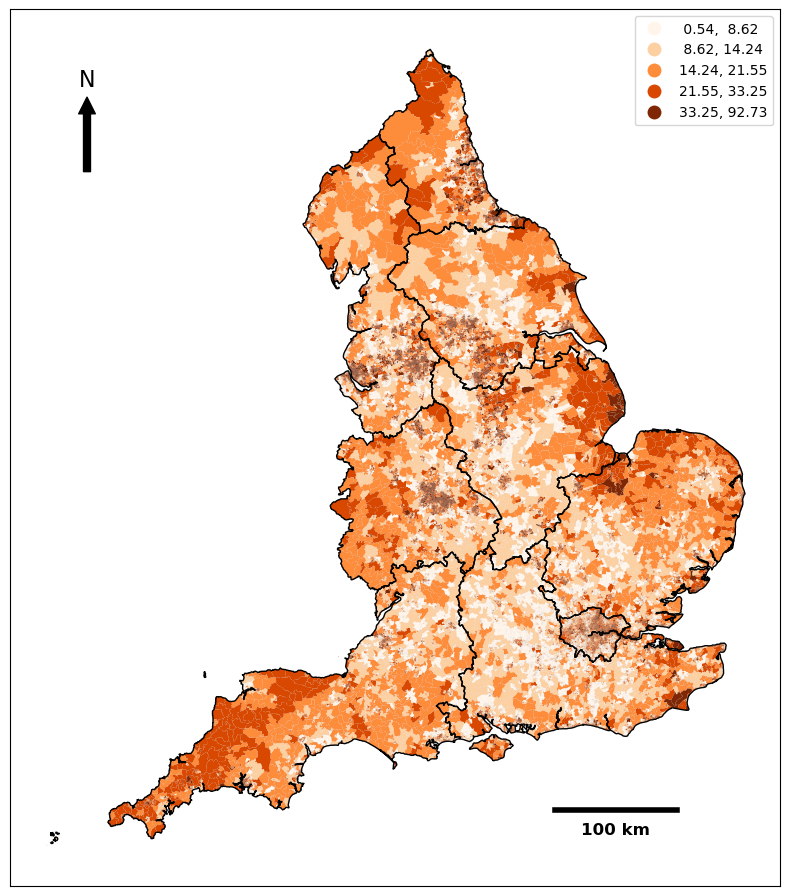
\includegraphics[width=1\linewidth]{ucl-latex-thesis-templates-master/Image/datageo_IMDLSOA_2.1.png}
  \caption{LSOA level.}
  \label{fig:A3.21}
\end{subfigure}%
\begin{subfigure}{.39\textwidth}
  \centering
  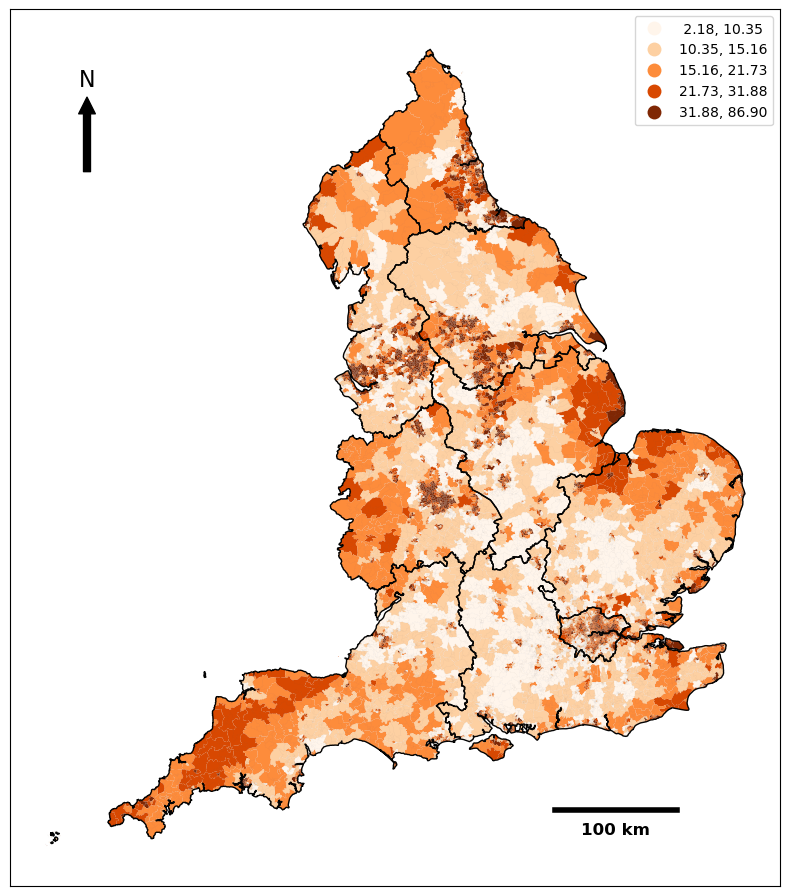
\includegraphics[width=1\linewidth]{ucl-latex-thesis-templates-master/Image/datageo_IMDMSOA_2.2.png}
  \caption{MSOA level.}
  \label{fig:A3.22}
\end{subfigure}
\caption{Maps comparing the geographical distribution of IMD scores at LSOA and MSOA levels.}
\label{fig:A3.2}
\end{figure}


\subsection{Lifestyle Group and Children Care}
\label{sec:3.2.4}
Based on the literature review, we found that unhealthy lifestyle habits such as drinking alcohol, smoking, and consuming sugary drinks are significant risk factors for diabetes. We collected corresponding datasets to represent variables in the lifestyle group. For alcohol misuse, we used the dataset provided by OHID, Hospital Admissions for Alcohol Attributable Conditions (2017), as a measure of alcohol abuse in different areas. This dataset calculates the standardized admission ratio for alcohol-related hospitalizations, with the numerator being alcohol-attributable admissions and the denominator being the expected number of admissions.
Smith et al. (2021) modeled dietary consumption among adults in England using small-area estimation methods. Their dataset, available at the MSOA level, aligns with our study's requirements. Their study focused on adults aged 16 and over, which matches our age group design. They calculated the average prevalence of adults consuming more than 330ml of sugar-sweetened beverages (SSBs) per day, a measure we will adopt.
For smoking behavior, we chose to use the prevalence of COPD, as Baker's project includes estimates of 20 health conditions, including COPD. According to NHS guidance (2022), around 90\% of COPD cases are smoking-related, with smoking being the primary cause. Given this strong correlation, we used COPD prevalence as an independent variable in the study, as it not only reflects smoking habits but also helps explore the connection between these two chronic conditions. Overweight status, another significant factor repeatedly mentioned in the literature, is measured at the MSOA level for obesity prevalence, also available from Baker's project. According to the OB002 indicator from the QOF 2022/23 guidance (NHS England, 2022), this obesity prevalence captures patients aged 18 and above with a BMI of 30 or higher, which fits our age group design.
We also included a variable reflecting child care using the Emergency admissions in children under five years old data provided by OHID (2023). This dataset calculates the number of completed emergency admissions as the numerator and the estimated population of children aged 0-4 as the denominator, multiplied by 1,000 to give a per-thousand rate. This dataset can highlight early health risk factors, helping us explore how early-life environments and childcare impact long-term health outcomes.


\subsection{Data Alignment for MSOA Boundary}
\label{sec:3.2.5}
It is important to note that our demographic variables are based on data from 2021 and beyond, using the 2021 MSOA boundaries. However, the other datasets, such as the 2019 IMD data, dietary studies using pre-2021 data, and various health data, all use the 2011 MSOA boundaries. Therefore, we standardized all datasets to the 2011 MSOA boundaries, as recalculating the other data to match the 2021 boundaries would be impractical due to the complexity of the calculations involved. The exact fit lookup file provided by ONS (2024) helps resolve this issue. The `CHNGIND’ column in the CSV file shows how the 2011 MSOAs were transformed into the 2021 MSOAs, categorizing the changes into four types: U (unchanged), S (split), M (merged), and X (mixed change). We found that 6,677 MSOAs remained unchanged. 75 2011 MSOAs were split into 155 2021 MSOAs, 32 were merged into 16, and 7 underwent complex changes, forming 8 2021 MSOAs. Using this lookup table, we can easily align our demographic dataset with the other datasets into a unified dataset.


\subsection{Project Code GitHub Repository}
\label{sec:3.2.6}
All the code for this project can be found at the following link: \url{https://github.com/ShengAric92/CASA0010_dissertation}, ensuring the reproducibility of the results. This project utilizes two programming languages, Python and R, for data processing, data analysis, and data visualization. The four Jupyter notebooks provided include `main\_data.ipynb', which demonstrates the entire data processing procedure, while the remaining notebooks display data visualization for each stage. Since the spatialreg package in R is highly effective for spatial regression analysis, R is used for data analysis in this project. Please refer to the `main\_methods\_spatial\_regression.qmd' file for details.


\section{Data Distribution}
\label{sec:3.3}
Figures \ref{fig:A3.3} and \ref{fig:A3.4}, respectively, show the histograms and Q-Q plots of all variables except the IMD decile to examine data distribution. We found that the variables within ethnic groups do not follow a normal distribution. Additionally, the following variables also do not conform to a normal distribution: Age17\_29, population density, children care (`Childrenemerg'), alcohol consumption (`Alcohol'), and high SSB consumption (`HighSSB'). Therefore, attention should be given to these variables in subsequent regression analyses, and appropriate data transformations, such as log transformation, may be necessary. The IMD decile variable is somewhat unique because deciles are a method that divides a distribution into ten equal parts, so it is not shown here. Furthermore, except for the IMD decile (considered as a continuous variable), population density (measured in people per hectare), `Childrenemerg', and `Alcohol', all other variables are expressed as percentages.

\begin{figure}[!ht]
  \centering
  
  % First figure
  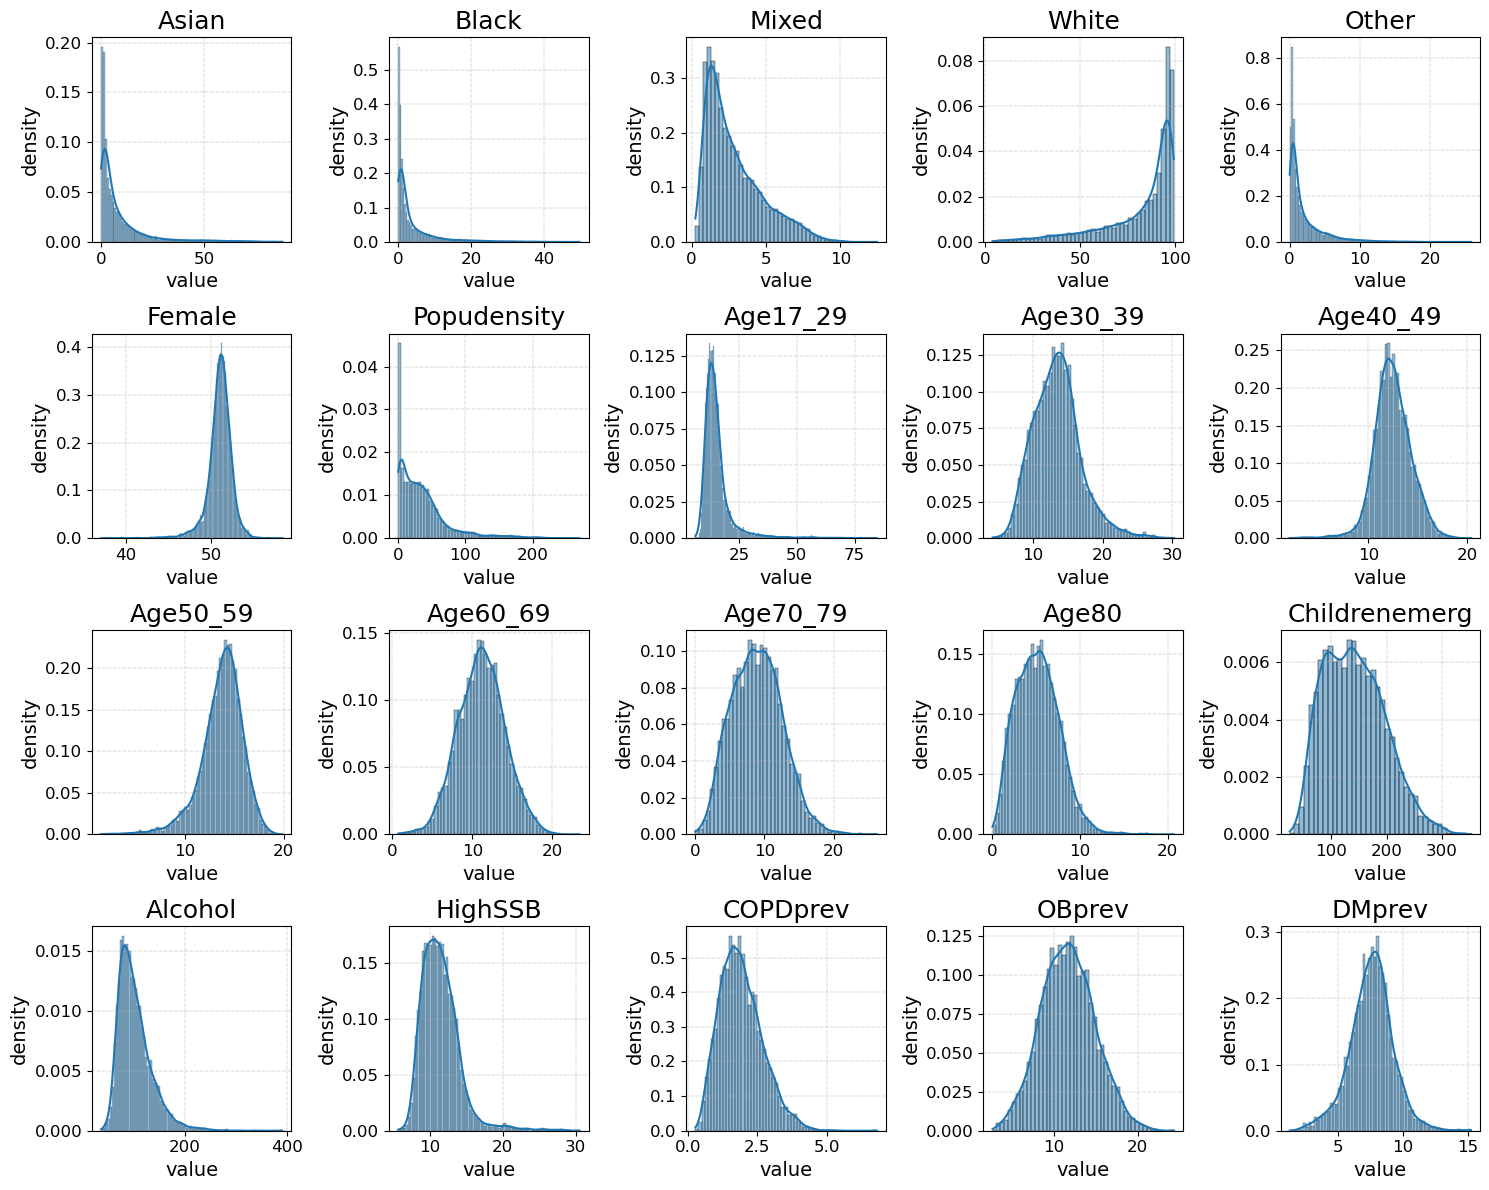
\includegraphics[width=.85\linewidth]{ucl-latex-thesis-templates-master/Image/data_hist_1.png}
  \caption{Histograms for All Variables (except IMD decile).}
  \label{fig:A3.3}
  
  \vspace{0.5cm} % Adjust vertical space between figures if needed
  
  % Second figure
  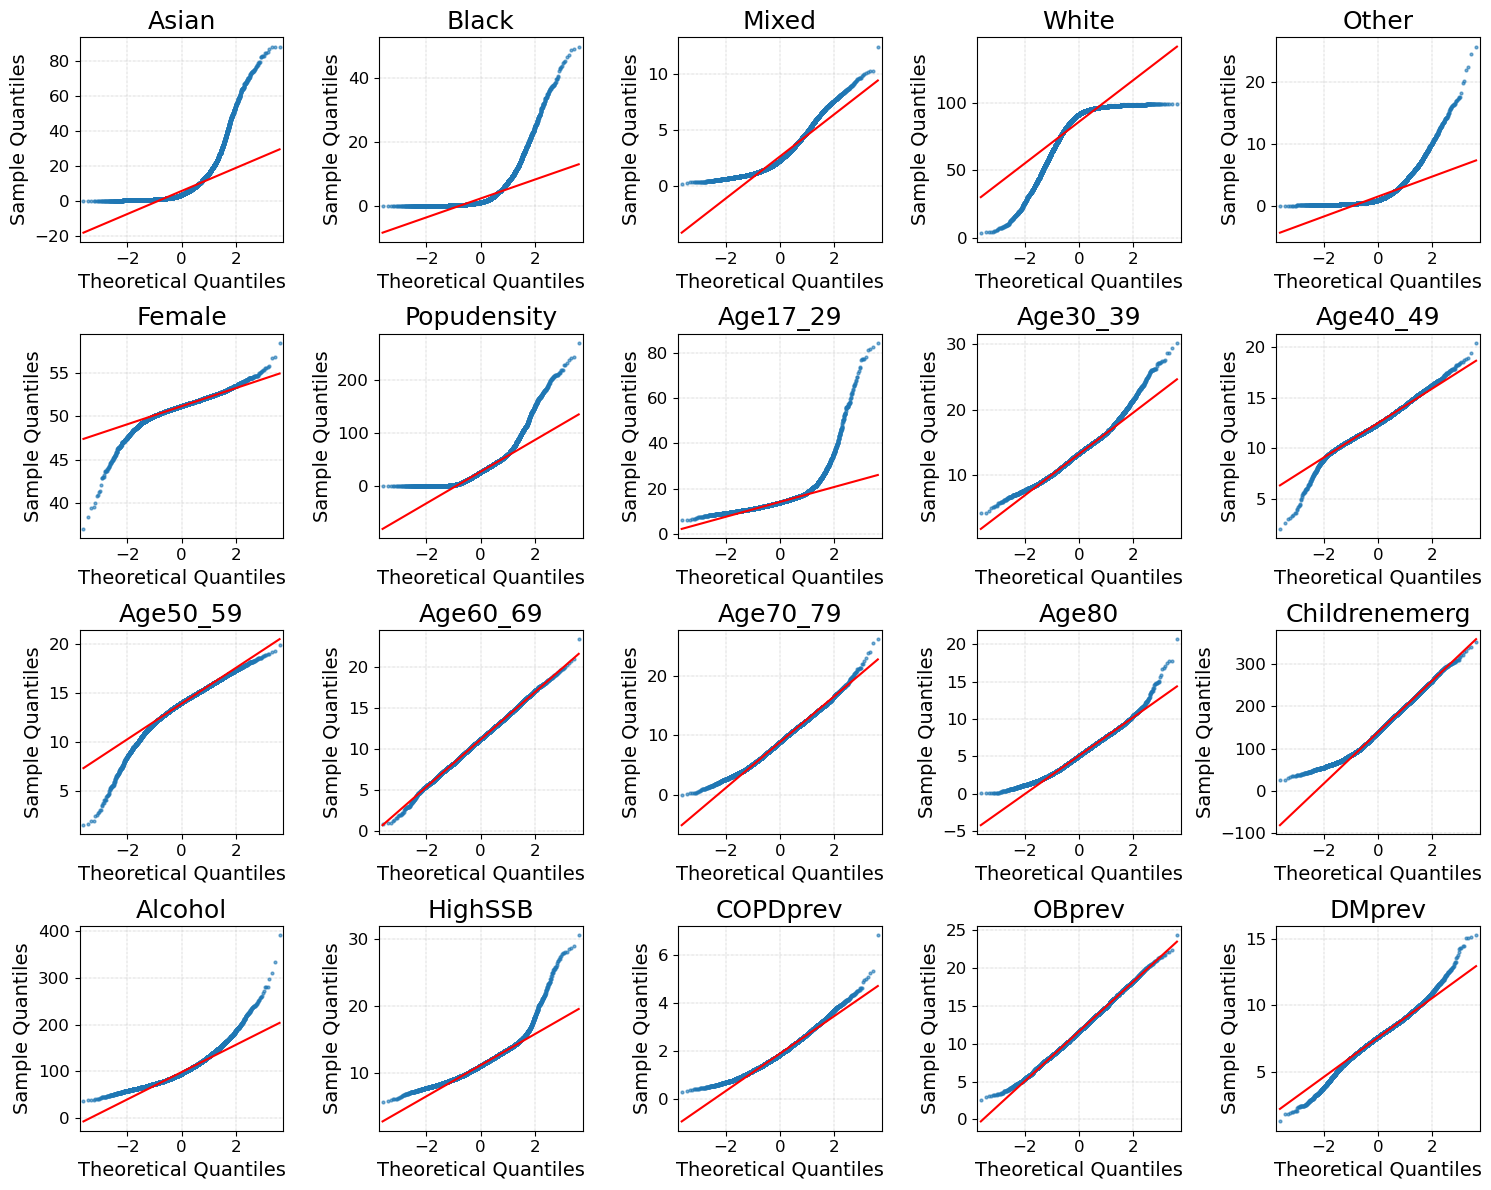
\includegraphics[width=.85\linewidth]{ucl-latex-thesis-templates-master/Image/data_qqplot_2.png}
  \caption{Q-Q Plots for All Variables (except IMD decile).}
  \label{fig:A3.4}
  
\end{figure}


\section{Methodology}
\label{sec:3.4}
To effectively address our research questions, this section will provide a methodology overview stage by stage.
\subsection{Exploratory Spatial Data Analysis}
\label{sec:3.4.1}
\subsubsection{Global Moran's I}
\label{sec:3.4.1.1}
Firstly, we need to explore the spatial distribution pattern of DM prevalence to determine whether it exhibits spatial clustering or dispersion. Therefore, the use of Global Moran's I is necessary, as it measures the degree of spatial autocorrelation of a variable across the entire study area. It is bounded by -1 and 1 and it is calculated using the form:
\begin{equation}
I=\frac{n}{s} \frac{\sum_{i=1}^n \sum_{j=1}^n w_{i j}\left(x_i-\bar{x}\right)\left(x_j-\bar{x}\right)}{\sum_{i=1}^n\left(x_i-\bar{x}\right)^2},
\end{equation}
where $n$ is the number of observations, $s$ is the sum of spatial weights, $\bar{x}$ is the mean of variable, and $w_{i j}$ denotes the spatial weight between observations index $i$ and $j$.

\subsubsection{Spatial Weights Matrix}
\label{sec:3.4.1.2}
This study uses Queen contiguity spatial weights to capture spatial interactions between neighboring areas. Given that the GP catchment areas at the MSOA level do not cover a large number of observations and that DM is a noncommunicable disease, which does not spread as rapidly as infectious diseases, K-Nearest Neighbours (KNN) spatial weights were ruled out. Additionally, the Isles of Scilly represent a special case, as the GP practice on the island provides medical services for the entire island. Thus, it is treated as an isolated unit and will employ a zero policy. Row normalization will be applied to meet the requirements for subsequent spatial dependence diagnostics and Monte Carlo Simulation.

\subsection{Correlation Analysis}
\label{sec:3.4.2}
Correlation analysis will be used to explore whether there is a linear relationship between variables. However, it’s important to remember that correlation does not imply causation. We will compute the Pearson correlation coefficient for each pair of variables to generate a sample correlation matrix. The entries of this matrix are defined by:

\begin{equation}
r_{i j}=\frac{\operatorname{cov}\left(v_i, v_j\right)}{\operatorname{sd}\left(v_i\right) * \operatorname{sd}\left(v_j\right)}=\frac{\sum_{l=1}^n\left(v_{i_l}-\bar{v}_i\right)\left(v_{j_l}-\bar{v}_j\right)}{\sqrt{\sum_{l=1}^n\left(v_{i_l}-\bar{v}_i\right)^2} \sqrt{\sum_{l=1}^n\left(v_{j_l}-\bar{v}_j\right)^2}},
\end{equation}
where $n$ is the size of observations, $v$ denotes the variable. IMD decile has been treated as a continuous variable, so it can also be used to calculate the Pearson correlation coefficient with other variables. Additionally, variables that are not significantly related to the dependent variable will be removed and excluded from the regression analysis.


\subsection{Regression Analysis: Ordinary Least Squares}
\label{sec:3.4.3}
\subsubsection{OLS Formula and Assumptions}
\label{sec:3.4.3.1}
To explore which risk factors significantly affect DM prevalence, we first established an Ordinary Least Squares (OLS) regression, with the following formula:
\begin{equation}
y=X \beta+\epsilon,
\end{equation}
where $y$ is the dependent variable, $X$ is the design matrix, $\beta$ is the vector of regression coefficients and $\epsilon$ is the error terms. In addition, the model must avoid multicollinearity and meet key assumptions, including homoscedasticity, independent errors, normally distributed errors, and exist a linear relationship. Therefore, the Durbin-Watson test, Jarque-Bera test, and Goldfeld-Quandt test will be used to assess whether the model meets these assumptions. Additionally, we use Z-score standardization to facilitate comparison between the regression coefficients.
\subsubsection{Variance Inflation Factor and Backward Elimination}
\label{sec:3.4.3.2}
In the age and ethnicity group variables, one variable from each group is manually removed as a reference variable to avoid multicollinearity. Additionally, the Variance Inflation Factor (VIF) is used to prevent multicollinearity, with a threshold set at 4 to avoid severe multicollinearity. To simplify the model, we also employed Backward Elimination (Marill and Green, 1963) to ensure that the remaining variables in the model are significant.
\subsubsection{Spatial Dependence Diagnostics}
\label{sec:3.4.3.3}
According to Anselin and Bera (1998), we know that OLS models are not always reliable because they do not account for spatial autocorrelation. Therefore, we need to perform spatial diagnostics on the OLS residuals, with Moran's I being used to test for spatial autocorrelation in the residuals. Suppose spatial autocorrelation is present in the residuals. In that case, we must then use spatial regression models such as the spatial lag model (SLM) or the spatial error model (SEM), and conduct Lagrange Multiplier (LM) tests and Robust LM tests to select the appropriate model. According to Anselin (2005), after performing the LM test, if either SLM or SEM is significant, the significant model should be chosen. If both models are significant, the Robust LM test is needed to select the appropriate model. If both models are significant in the Robust LM test, the model with the larger test statistic should be chosen.


\subsection{Spatial Regression Analysis}
\label{sec:3.4.4}
According to the studies by Osayomi (2019) and Turi (2017), three common spatial regression models are widely used in spatial epidemiology. These models are the spatial lag model (SLM), the spatial error model (SEM), and the spatial Durbin model (SDM). This subsection will introduce each of these three models.
\subsubsection{Spatial Lag Model}
\label{sec:3.4.4.1}
The SLM focuses on the spatial lag effect of the dependent variable, capturing whether the dependent variable in an area is influenced by the dependent variables in neighboring areas. Its formula is as follows:
\begin{equation}
y=\rho W y+X \beta+\epsilon.
\end{equation}
Here $\rho$ is the spatial lag coefficient, $W$ is the spatial weight matrix, $\beta$ is the regression coefficients vector and $\epsilon$ is the error term. $\rho W y$ is the added spatially lagged value, and due to the inclusion of this term, the SLM cannot be directly compared with OLS. Generally, we need to calculate the direct effect and the indirect effect in the model.
\subsubsection{Spatial Error Model}
\label{sec:3.4.4.2}
The SEM can handle spatial autocorrelation in the error terms. It can reveal clusters of unexplained spatially correlated values in neighbouring areas caused by omitted variables that were not included in the model. Its formula is as follows:
\begin{equation}
y=X \beta+u, \quad u=\lambda W u+\epsilon.
\end{equation}
Here $u$ is the function of unexplained residuals and neighbors residuals, where $\lambda$ measures the correlation between neighbouring residuals.
\subsubsection{Spatial Durbin Model}
\label{sec:3.4.4.3}
SLM and SEM can only capture part of the spatial dependency, whereas the SDM combines the considerations of both models. It can simultaneously capture the spatial lag effects of both the dependent and independent variables and helps to identify the spatial spillover effect of the independent variables, which is the impact of the independent variables in neighboring areas on the dependent variable in the current area. Its formula is:
\begin{equation}
y=\rho W y+X \beta+W X \theta+\epsilon.
\end{equation}
We need to note that the spatially lagged value of the independent variables is also included, where $\theta$ is the vector of spatially lagged independent variables' coefficients. Therefore, like the SLM, this model also requires the calculation of both the direct effect and the indirect effect of the variables.

\subsection{Model Selection and Comparison}
\label{sec:3.4.5}
\subsubsection{SDM Degenerate Test}
\label{sec:3.4.5.1}
Some economists and ecologists have started to expand the use of spatial regression models, suggesting that if both SLM and SEM remain highly significant after performing a Robust LM test, a more comprehensive model should be considered. For example, the studies by Patnaik (2023) and Shang (2024) used the Likelihood Ratio (LR) test to determine whether the SDM could degenerate into an SLM or SEM. If the LR test for both models is still highly significant with the SDM, it indicates that the SDM cannot be simplified to an SLM or SEM. Of course, the final choice should also consider the performance of these models and their relevance to real-world situations.
\subsubsection{Model Comparison}
\label{sec:3.4.5.2}
To compare the models, the Akaike Information Criterion (AIC) and the Bayesian Information Criterion (BIC) will be used. These two metrics assess the goodness of fit of the models, with lower AIC and BIC values indicating better model fit. Additionally, it is necessary to test for spatial autocorrelation in the model residuals, using Moran's I for diagnostic testing. If the model effectively removes spatial autocorrelation in the residuals, it indicates that the model has successfully captured and addressed the spatial dependencies in the data.

\section{Ethical evaluation}
\label{sec:3.5}
The ethical risk level of this project is considered minimal and does not require further ethical review, as all datasets used are openly available and can be easily downloaded free of charge. The data were sourced from various online platforms run by government agencies, such as demographic data from the ONS and public health data from NHS Digital and OHID. These datasets are provided under the Open Government Licence, the details of which can be found at this link: \url{https://www.nationalarchives.gov.uk/doc/open-government-licence/version/3/}. The availability of these data supports academic research, encourages innovation, and provides support and evidence for the development of public health policy.

This project also utilizes data based on research and other research projects. For example, Smith et al. (2021) estimated fruit, vegetable, and SSB consumption data in their study on adult dietary habits in England. Baker's project (2021) transformed the QOF's publicly available GP-level prevalence data for various conditions into estimated area-level prevalence data. The datasets produced by these two projects are available under the Creative Commons Attribution License (details here: \url{https://creativecommons.org/licenses/by/4.0/}) and the Open Parliament Licence (details here: \url{https://www.parliament.uk/site-information/copyright-parliament/open-parliament-licence/}), respectively. By making their research findings available online as open data, they uphold academic transparency and facilitate further research and reuse of the data. This aligns with the core values of transparency and inclusivity in health data science, as highlighted by Ford et al. (2019). This project has used these datasets correctly and cautiously, with careful and appropriate citation.

It is important to note that the method for estimating prevalence rates incorporates data on the distribution of patients at the LSOA level, publicly provided by the NHS for each GP. Since January 2020, the NHS has published quarterly reports on the distribution of GP patients (NHS England, 2020). The NHS ensures that these data are anonymized and do not include any patient address information, which aligns with Tene and Polonetsky's (2012) emphasis on balancing individual privacy with the beneficial use of data. Accordingly, this project's datasets and analyses do not involve personal or sensitive information.